\PassOptionsToPackage{unicode=true}{hyperref} % options for packages loaded elsewhere
\PassOptionsToPackage{hyphens}{url}
%
\documentclass[12pt,]{report}
\usepackage{lmodern}
\usepackage{amssymb,amsmath}
\usepackage{ifxetex,ifluatex}
\usepackage{fixltx2e} % provides \textsubscript
\ifnum 0\ifxetex 1\fi\ifluatex 1\fi=0 % if pdftex
  \usepackage[T1]{fontenc}
  \usepackage[utf8]{inputenc}
  \usepackage{textcomp} % provides euro and other symbols
\else % if luatex or xelatex
  \usepackage{unicode-math}
  \defaultfontfeatures{Ligatures=TeX,Scale=MatchLowercase}
\fi
% use upquote if available, for straight quotes in verbatim environments
\IfFileExists{upquote.sty}{\usepackage{upquote}}{}
% use microtype if available
\IfFileExists{microtype.sty}{%
\usepackage[]{microtype}
\UseMicrotypeSet[protrusion]{basicmath} % disable protrusion for tt fonts
}{}
\IfFileExists{parskip.sty}{%
\usepackage{parskip}
}{% else
\setlength{\parindent}{0pt}
\setlength{\parskip}{6pt plus 2pt minus 1pt}
}
\usepackage{hyperref}
\hypersetup{
            pdftitle={Geometría diferencial},
            pdfauthor={Ricardo Michel MALLQUI BAÑOS},
            pdfborder={0 0 0},
            breaklinks=true}
\urlstyle{same}  % don't use monospace font for urls
\usepackage{longtable,booktabs}
% Fix footnotes in tables (requires footnote package)
\IfFileExists{footnote.sty}{\usepackage{footnote}\makesavenoteenv{longtable}}{}
\usepackage{graphicx,grffile}
\makeatletter
\def\maxwidth{\ifdim\Gin@nat@width>\linewidth\linewidth\else\Gin@nat@width\fi}
\def\maxheight{\ifdim\Gin@nat@height>\textheight\textheight\else\Gin@nat@height\fi}
\makeatother
% Scale images if necessary, so that they will not overflow the page
% margins by default, and it is still possible to overwrite the defaults
% using explicit options in \includegraphics[width, height, ...]{}
\setkeys{Gin}{width=\maxwidth,height=\maxheight,keepaspectratio}
\setlength{\emergencystretch}{3em}  % prevent overfull lines
\providecommand{\tightlist}{%
  \setlength{\itemsep}{0pt}\setlength{\parskip}{0pt}}
\setcounter{secnumdepth}{5}

% set default figure placement to htbp
\makeatletter
\def\fps@figure{htbp}
\makeatother

\usepackage{etoolbox}
\makeatletter
\providecommand{\subtitle}[1]{% add subtitle to \maketitle
  \apptocmd{\@title}{\par {\large #1 \par}}{}{}
}
\makeatother
\usepackage[spanish,es-noquoting]{babel}
\usepackage[utf8]{inputenc}
\usepackage{amsfonts}
\usepackage[T1]{fontenc}
\usepackage{booktabs,longtable}
\usepackage[referable]{threeparttablex}
\usepackage{dsfont}
\usepackage[a4paper]{geometry}
\geometry{verbose,tmargin=2.5cm,bmargin=2.5cm,lmargin=3cm,rmargin=2.5cm}
\usepackage{booktabs}
\renewcommand{\rmdefault}{ptm}
\usepackage[lite,subscriptcorrection,nofontinfo,zswash]{mtpro2}
\usepackage{textcase}
\usepackage{makecell}
\usepackage{lscape}
\usepackage{multirow}
\usepackage{tabto}
\usepackage{bigstrut}
\usepackage{titlesec}
\DeclareFontFamily{U}{mt2ms}{\skewchar\font42}%
\DeclareFontShape{U}{mt2ms}{m}{n}{<-7>mt2mcf<7-9>mt2mcs<9->mt2mct}{}%
\DeclareFontShape{U}{mt2ms}{m}{it}{<-7>mt2msf<7-9>mt2mss<9->mt2mst}{}%
\DeclareFontShape{U}{mt2ms}{b}{it}{<-7>mt2bmsf<7-9>mt2bmss<9->mt2bmst}{}%

\usepackage{showframe}

%\usepackage{fancyhdr}
%\pagestyle{fancyplain}
%\fancyhf{}
%\fancyhead[R]{\thepage}
%\renewcommand{\headrulewidth}{0pt}
%\setlength{\headheight}{2.5 cm}
\titlespacing*{\chapter}
{0pt} {9em plus .01em minus .01em} {0em plus .01em minus .01em}
\titlespacing*{\section}
{0pt} {0em plus .01em minus .01em} {0em plus .01em minus .01em}
\titlespacing*{\subsection}
{0pt} {0em plus .01em minus .01em} {0em plus .01em minus .01em}
\titlespacing*{\subsubsection}
{0pt} {0em plus .01em minus .01em} {0em plus .01em minus .01em}
\titlespacing*{\paragraph} {0pt}{1.25ex plus 1ex minus .2ex}{2em}
\titlespacing*{\subparagraph} {\parindent}{3.25ex plus 1ex minus .2ex}{1em}
\titleformat*{\section}{\normalsize\bfseries}
\titleformat*{\subsection}{\normalsize\bfseries}
\setlength{\parskip}{0.7em plus .01em minus .01em}
%%%%%%


\usepackage{amsthm}
\newtheoremstyle{slplain}% name
  {0.5em plus 0.01em minus 0.01em}% Space above
  {0em plus 0.01em minus 0.01em}% Space below
  {\slshape}% Body font
  {}%Indent amount (empty = no indent, \parindent = para indent)
  {\bfseries}%  Thm head font
  {......}%       Punctuation after thm head
  { }%      Space after thm head: " " = normal interword space;
        %       \newline = linebreak
  {}%       Thm head spec


\theoremstyle{slplain}
\newtheorem{thm}[equation]{Theorem}  % Numbered with the equation counter
\newtheorem{cor}[equation]{Corollary}     
\newtheorem{lem}[equation]{Lemma}         
\newtheorem{prop}[equation]{Proposition}
\newtheorem{theorem}{Teorema}[chapter]
\newtheorem{lemma}{Lema}[chapter]
\newtheorem{corollary}{Corolario}[chapter]
\newtheorem{proposition}{Proposición}[chapter]
\newtheorem{conjecture}{Conjectura}[chapter]
\newtheorem{definition}{Definición}[chapter]
\newtheorem{example}{Ejemplo}[chapter]
\newtheorem{exercise}{Ejercicio}[chapter]
\newtheorem*{remark}{Observación}
\newtheorem*{solution}{Solución}

%%%%%%%%%%%%%%%%%%%%%%%%%%
\usepackage{xpatch}%space equation
\xapptocmd\normalsize{%
\abovedisplayskip=0.5em plus 0.01em minus 0.01em
\abovedisplayshortskip=0.5em plus 0.01em minus 0.01em
\belowdisplayskip=0.5em plus 0.01em minus 0.01em
\belowdisplayshortskip=0.5em plus 0.01em minus 0.01em
}{}{}
%%%%%%%%%%%%%%%%%%%%%

\usepackage{url}

%\usepackage{breakurl}
\usepackage{chngcntr}
\renewcommand{\thefigure}{\arabic{chapter}.\arabic{figure}}
\renewcommand{\thetable}{\arabic{chapter}.\arabic{table}}
\renewcommand{\theequation}{\arabic{section}.\arabic{equation}}

\usepackage{amsthm}
\usepackage{chngcntr} 
%\newtheorem{thm}{Theorem}[subsection]
%\newtheorem{theorem}{Teorema}[section]
%\renewcommand{\thetheorem}{\arabic{section}.\arabic{theorem}}
%\renewcommand{\thetheorem}{\arabic{chapter}.\arabic{theorem}}

%\renewcommand{\thechapter}{\Roman{chapter}}

\titleformat{\chapter}[display]
{\normalfont\normalsize\bfseries}{CAPÍTULO \thechapter}{0.0em}{\normalsize\bfseries}
%\renewcommand{\thechapter}{\Roman{chapter}}
\renewcommand{\thesection}{\arabic{chapter}.\arabic{section}}
\renewcommand{\thesubsection}{\arabic{chapter}.\arabic{section}.\arabic{subsection}}
\renewcommand{\thesubsubsection}{\arabic{chapter}.\arabic{section}.\arabic{subsection}.\arabic{subsubsection}}
\flushbottom
% https://github.com/rstudio/rmarkdown/issues/337
\let\rmarkdownfootnote\footnote%
\def\footnote{\protect\rmarkdownfootnote}

% https://github.com/rstudio/rmarkdown/pull/252
\usepackage{titling}
\setlength{\droptitle}{-2em}

\pretitle{\vspace{\droptitle}\centering\huge}
\posttitle{\par}

\preauthor{\centering\large\emph}
\postauthor{\par}

\predate{\centering\large\emph}
\postdate{\par}
\usepackage[]{natbib}
\bibliographystyle{apalike}

\title{Geometría diferencial}
\author{Ricardo Michel MALLQUI BAÑOS}
\providecommand{\institute}[1]{}
\institute{Universidad Nacional San Cristóbal De Huamanga}
\date{2020-02-17}

\let\BeginKnitrBlock\begin \let\EndKnitrBlock\end
\begin{document}
\maketitle

{
\setcounter{tocdepth}{1}
\tableofcontents
}
\newcommand{\N}{\mathbb{N}}
\newcommand{\R}{\mathbb{R}}
\newcommand{\CC}{\mathbb{C}}
\newcommand{\I}{\mathbb{I}}
\newcommand{\f}{\mathbb{f}}
\newcommand{\X}{\mathbb{X}}
\newcommand{\D}{\mathbb{D}}
\newcommand{\Z}{\mathbb{Z}}
\newcommand{\Q}{\mathbb{Q}}
\newcommand{\norm}[1]{\left\Vert#1\right\Vert}
\newcommand{\abs}[1]{\left\vert#1\right\vert}
\newcommand{\set}[1]{\left\{#1\right\}}
\newcommand{\seq}[1]{\left<#1\right>}
\newcommand{\co}[1]{\left[#1\right]}
\newcommand{\cc}[1]{\left(#1\right)}
\newcommand{\J}{\mathcal{J}}
\newcommand{\K}{\mathcal{K}}
\newcommand{\M}{\mathcal{M}}
\newcommand{\F}{\mathcal{F}}

\hypertarget{prerequisitos}{%
\chapter{Prerequisitos}\label{prerequisitos}}

\hypertarget{ingresar-imagen}{%
\section{Ingresar imagen}\label{ingresar-imagen}}

Generar pdf y svg en inskape(ajustar Shift+Ctrl+R) o relativos luego se debe guardar en el mismo directorio general luego se usa el entorno \texttt{ff\ fff}
\[\prod_1^2\]
\#\#\# Vector

\[\vec{w}\]

\hypertarget{recta}{%
\subsection{Recta}\label{recta}}

See Theorem \ref{thm:boring}

\begin{figure}

{\centering 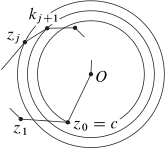
\includegraphics{inverse} 

}

\caption{ww}\label{fig:pressure2}
\end{figure}

Here is my theorem.
Here is my theorem.

\BeginKnitrBlock{theorem}
\protect\hypertarget{thm:boring}{}{\label{thm:boring} }Here is my theorem. Here is my theorem.
Here is my theorem.
Here is my theorem.
Here is my theorem.
Here is my theorem.
Here is my theorem.
\EndKnitrBlock{theorem}

sea Here is my theorem.
Here is my theorem.
Here is my theorem.
Here is my theorem.
Here is my theorem.

\BeginKnitrBlock{definition}[ww]
\protect\hypertarget{def:unnamed-chunk-1}{}{\label{def:unnamed-chunk-1} \iffalse (ww) \fi{} }Sea la siguiente formula Here is my theorem.
Here is my theorem.
Here is my theorem.
Here is my theorem.
Here is my theorem.
\EndKnitrBlock{definition}

\begin{figure}

{\centering 
\includegraphics[width=0.2\linewidth]{U} 

}

\caption{ww}\label{fig:pressure1}
\end{figure}

Here is my theorem.
Here is my theorem.
Here is my theorem.

\hypertarget{intro}{%
\chapter{Introduction}\label{intro}}

\citep{xie2015}

\hypertarget{literature}{%
\chapter{Literature}\label{literature}}

Here is a review of existing methods.

\hypertarget{methods}{%
\chapter{Methods}\label{methods}}

We describe our methods in this chapter.

\hypertarget{applications}{%
\chapter{Applications}\label{applications}}

Some \emph{significant} applications are demonstrated in this chapter.

\hypertarget{example-one}{%
\section{Example one}\label{example-one}}

\hypertarget{example-two}{%
\section{Example two}\label{example-two}}

\hypertarget{final-words}{%
\chapter{Final Words}\label{final-words}}

We have finished a nice book.

\bibliography{book.bib}

\end{document}
